\documentclass[12pt]{article}
\usepackage{fancyhdr,lastpage}
\usepackage{multicol}
\usepackage{graphicx}
\usepackage{amssymb}
\usepackage{epstopdf}
\DeclareGraphicsRule{.tif}{png}{.png}{`convert #1 `basename #1 .tif`.png}

\textwidth = 6.5 in
\textheight = 10 in
\oddsidemargin = 0.0 in
\evensidemargin = 0.0 in
\topmargin = 0.0 in
\headheight = 0.0 in
\headsep = 0.0 in
\parskip = 0.2in
\parindent = 0.0 in
\pagestyle{fancy}

\lhead{Physics 12\\Rick Kidd}
\rhead{Steffen L. Norgren\\May 8$^{th}$, 2003}

\begin{document}

\begin{center}
	\footnotesize{Created using \LaTeX\ }
	\paragraph{}
	\LARGE{\textbf{\underline{Momentum Oblique Collision Lab}}}
\end{center}

\section{Purpose \& Data Presentation}

In this experiment we will investigate a model of elastic collision, checking theoretical predictions against experimental data for conservation of momentum.
	
Height of Table ($h$): \textbf{0.8933 m}\newline
Mass of Ball-Bearing A ($m_{a}$): \textbf{0.028041 kg}\newline
Mass of Ball-Bearing B ($m_{b}$): \textbf{0.027873 kg}

The uncollided trial run was conducted using only ball-bearing A. The experiment involving a collision was conducted such that ball-bearing A struck ball-bearing B, which was situated at the bottom of the ramp and slightly offset as to product two angled resultant trajectories. See attached diagram for experimental results.

Range of Uncollided Ball-Bearing A ($m_{a}$): \textbf{0.3320 m}

The results of the trial run using ball-bearing A were used to define the x-axis from which we could measure the angles of the resultant trajectories from the ball-bearing collisions. The angles measured are using a best-fit line for multiple collisions. All angles are measured with respect to the x-axis.

Range and Angle ($\angle \alpha$) of Collided Ball-Bearing A ($m_{a}$): \textbf{0.1670 m @ 11.1$^{\circ}$}\newline
Range and Angle ($\angle \beta$) of Collided Ball-Bearing B ($m_{b}$): \textbf{0.2735 m @ -18.0$^{\circ}$}

With the distance (range) and angles known, we can figure out the distance the objects travelled in the x and y directions as components. For these calculations, we will take $\angle \beta$ to be negative and $\angle \alpha$ to be positive.

For Ball-Bearing A ($m_{a}$):
\begin{equation}
d_{x_{a}}=(0.1670m)\cos11.1^{\circ}=0.163\overline{8}75m
\end{equation}
\begin{equation}
d_{y_{a}}=(0.1670m)\sin11.1^{\circ}=0.0321\overline{5}11m
\end{equation}

For Ball-Bearing B ($m_{b}$):
\begin{equation}
d_{x_{b}}=(0.2735m)\cos-18.0^{\circ}=0.260\overline{1}13m
\end{equation}
\begin{equation}
d_{y_{b}}=(0.2735m)\sin-18.0^{\circ}=-0.0845\overline{1}61m
\end{equation}

\pagebreak
\paragraph{}

\section{Calculations}
\begin{enumerate}
\item{
The horizontal velocity for both the collided and uncollided ball-bearings can be easily determined when one has the recorded the height of the table from which the object fell and the distance (range) that the object travelled from the point of origin at the table. Since vertical acceleration is pretermined by gravity, we know how long it takes the object to fall a measured distance. By finding the time that it takes the object to fall from the table, we can then find the initial and final horizontal velocity of the object based its range. The initial and final horizontal velocities should be the same as the effects of air friction is negligible in this experiment.

The time it takes an object to fall a certain distance can be derived with $t=\sqrt{\frac{2(h)}{g}}$ and the horizontal velocity of the object can be derived with $v_{a_{0}}=\frac{d}{t}$. We can combine these two formulas into a single formula $v_{a_{0}}=\frac{d}{\sqrt{\frac{2(h)}{g}}}$, which simplifies to:

\begin{equation}
v_{a_{0}}=\sqrt{\frac{gd^2}{2h}}
\end{equation}

Now we can plug in the height and distance (range) results from the experiment to come up with an initial and final horizontal velocity for the uncollided ball-bearing A ($m_{a}$):

\begin{equation}
v_{a_{0}}=\sqrt{\frac{9.80\frac{m}{s^2}(0.3320 m)^2}{2(0.8933 m)}}=0.777\overline{5}66\frac{m}{s}
\end{equation}}

\item{
Now that we know the initial and, therefore, final horizontal velocities, we can calculate the initial momentum for the uncollided ball-bearing A ($m_{a}$):

\begin{equation}
P_{a_{0}}=m_{a}v_{x}=(0.028041kg)(0.777\overline{5}66\frac{m}{s})=0.0218\overline{0}37kg\frac{m}{s}
\end{equation}}
\pagebreak
\space
\newline

\item{
Since we have made a best-fit line to average the results of several trials, we only need to make calculations based on measurements of the best fit line.

Velocity for Ball-Bearing A (from point of collision):
\begin{equation}
v_{a_{f}}=\sqrt{\frac{gd_{a}^2}{2h}}=\sqrt{\frac{9.80\frac{m}{s^2}(0.1670 m)^2}{2(0.8933 m)}}=0.391\overline{1}25\frac{m}{s}@ 11.1^{\circ}
\end{equation}

Velocity for Ball-Bearing B (from point of collision):
\begin{equation}
v_{b_{f}}=\sqrt{\frac{gd_{b}^2}{2h}}=\sqrt{\frac{9.80\frac{m}{s^2}(0.2735 m)^2}{2(0.8933 m)}}=0.640\overline{5}55\frac{m}{s}@ -18.0^{\circ}
\end{equation}

Momentum for Ball-Bearing A (from point of collision):
\begin{equation}
P_{a_{f}}=m_{a}v_{a_{f}}=(0.028041kg)(0.391\overline{1}25\frac{m}{s})=0.0109\overline{6}75kg\frac{m}{s}
\end{equation}

Momentum for Ball-Bearing B (from point of collision):
\begin{equation}
P_{b_{f}}=m_{b}v_{b_{f}}=(0.027873kg)(0.640\overline{5}55\frac{m}{s})=0.0178\overline{5}42kg\frac{m}{s}
\end{equation}}
\pagebreak
\space
\newline

\item{
I have decided to calculate the resultant momentum by using a vector addition polygon where we find the resulting by using the sine and cosine laws. Theoretically the $\sum{P_{r}}$ should equal the initial $P_{a_{0}}$ for the uncollided ball-bearing A. The law of conservation of momentum states that $m_{1}v_{1}+m_{2}v_{2}=m_{1}v_{3}+m_{2}v_{4}$, that is that the sum of the initial momenta should equal the sum of the final momena. In our experiment ball-bearing B does not have any initial momentum as it has no velocity, therefore the initial momentum for ball-bearing A will be distributed between ball-bearing A \& B for the resulting momenta.

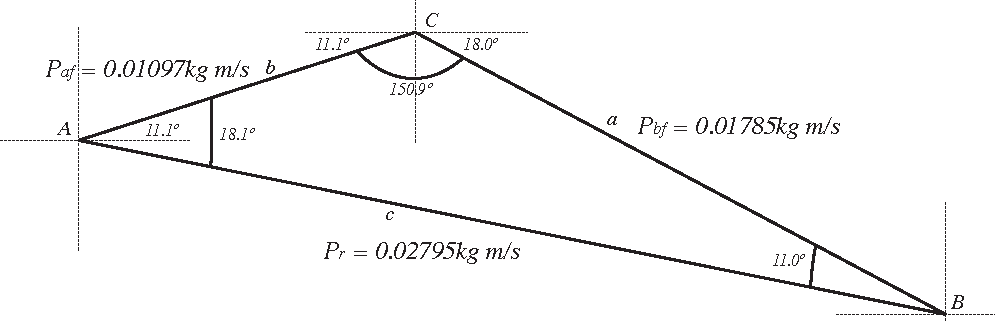
\includegraphics{polygon.pdf}

We use the cosine law to find the resultant momentum $P_{r}$

\begin{equation}
c^2=a^2+b^2-2ab\cos{C}
\end{equation}
\begin{equation}
c^2=(0.0178\overline{5}42kg\frac{m}{s})^2+(0.0109\overline{6}75kg\frac{m}{s})^2-2(0.0178\overline{5}42kg\frac{m}{s})(0.0109\overline{6}75kg\frac{m}{s})\cos{150.9^{\circ}}
\end{equation}
\begin{equation}
P_{r}=c=\sqrt{0.000781\overline{2}56kg\frac{m}{s}}=0.0279\overline{5}10kg\frac{m}{s}
\end{equation}

Therefore the resultant of the two final momenta, $P_{r}=0.02795kg\frac{m}{s}$

Now we can use the sine law to find the unknown angles.

\begin{equation}
\frac{\sin{C}}{c}=\frac{\sin{B}}{b}
\end{equation}
\begin{equation}
\frac{\sin{150.9^{\circ}}}{0.0279\overline{5}10kg\frac{m}{s}}=\frac{\sin{B}}{0.0109\overline{6}75kg\frac{m}{s}}
\end{equation}
\begin{equation}
B=\sin^{-1}\frac{(0.0109\overline{6}75kg\frac{m}{s})\sin{150.9^{\circ}}}{0.0279\overline{5}10kg\frac{m}{s}}=11.\overline{0}01^{\circ}
\end{equation}

Now that we know two of the three angles in the polygon all we need to do is subtract the known angles from $180^{\circ}$ to determine the angle for $A$; therefore, $A=180.0^{\circ}-150.9^{\circ}-11.0^{\circ}=18.1^{\circ}$.}
\pagebreak
\space
\newline

\item{
To find the percent difference we use the following formula:
\begin{equation}
\%diff=\frac{experimental-true}{true}\times 100\%
\end{equation}
Where the experimental value is the resultant of the two momenta after collision, $P_{r}$, and the true value is the initial momentum for the uncollided ball-bearing A, $P_{a_{0}}$.
\begin{equation}
\%diff=\frac{P_{r}-P_{a_{0}}}{P_{a_{0}}}\times 100\%=\frac{0.0279\overline{5}10kg\frac{m}{s}-0.0218\overline{0}37kg\frac{m}{s}}{0.0218\overline{0}37kg\frac{m}{s}}\times 100\%=28.\overline{1}93\%
\end{equation}
Based on a rather large $28.2\%$ difference between the initial and final momenta, one can only conclude that this is due to some source of error in the experiment. Either the experiment did not remain static throughout all the trials, or somewhere a rather grievous calculation error has been made.}
\end{enumerate}

\section{Questions}
\begin{enumerate}

\item{
The diameter of the ball-bearings do not have any affect on the height measurement of the system, as is is the bottom of the ball-bearing that leaves the ledge first and it is the bottom of the ball-bearing that also hits the ground first.}

\item{
The limits of precision in the mass, displacement and momentum data are as follows (using only one representative value from each set of values):

$Height=0.8933m\pm0.0005m$\newline
\begin{equation}
\frac{0.0005m}{0.8933m}\times 100\%=0.056\%
\end{equation}

$Mass=0.028041kg\pm0.000001kg$\newline
\begin{equation}
\frac{0.000001kg}{0.028041kg}\times 100\%=0.0036\%
\end{equation}

$Displacement=0.3320m\pm0.0005m$\newline
\begin{equation}
\frac{0.0005m}{0.3320m}\times 100\%=0.15\%
\end{equation}

$Momentum=0.02180kg\frac{m}{s}\pm0.00005kg\frac{m}{s}$\newline
\begin{equation}
\frac{0.00005kg\frac{m}{s}}{0.02180kg\frac{m}{s}}\times 100\%=0.23\%
\end{equation}}
\pagebreak
\space
\newline

\item{
The reason the "initial momentum before collision" was needed was so that we could use the results of that trial as a baseline for where the x-axis was and so that we would have some data from which we could calculate the initial momentum, which was crucial to calculating the resultant momenta of the collided ball-bearings.}

\item{
The "initial momentum before collision" was the real momentum for the ball-bearing used in that trial, as we were able to determine the initial velocity of the trial ball-bearing based on the results of the trial experiment. As a result of the trial we had height and distance (range) data from which we can extrapolate the time needed for the object to fall and therefore the initial velocity as we also knew the distance the object travelled in said time.}

\item{
The factors that were controlled in this experiment was acceleration due to gravity ($9.80\frac{m}{s^2}$), the height of the table (unless you count changing tables), and therefore the time taken for the object to fall. Other factors that were kept constant include the masses of the ball-bearings and their elasticity.

The independent variables in this experiment included the height up the ramp that we released the ball-bearing, the angle at which the two ball-bearings collided, which ball-bearing was released from the ramp, and which ball-bearing was situated at the bottom of the ramp to be collided with. The reason I consider the arrangement of which ball-bearing hit which, is because they have slightly different masses, which would slightly affect the outcome of the experiment.}

\item{
There were many sources of error that could have affected the results of this experiment, as we can see by the horribly large percent difference between the initial and resultant momenta. The placement and angle of the ramp respective to the edge of the table is one major source of error. There is a good chance that the ramp's placement may have been slightly adjusted after the initial uncollided trial, which would affect the analysis of the results. Another source of error could be due to the paper slip that was situated at the end of the ramp, as it was in place during the trial run, but it was subsequently moved to ensure an angled collision that would actually have both ball-bearings land on the paper. The last major source of error could be due to the height up the ramp from which the ball-bearings were released. There is only a small chance that any significant measurement error occurred when we measured the resulting angles, masses of the ball-bearings, or the height of the table, as I took great care to take those measurements accurately.}

\end{enumerate}
\end{document}